
This Chapter returns to the Poisson equation in two dimensions.  We implement a finite element method (FEM) for an unstructured triangular mesh which covers a general polygonal domain.  Our code solves certain nonlinear generalizations of the standard linear problem, but these are different nonlinear forms from the $p$-Laplacian problem in the previous Chapter.

Our approach is to
\begin{center}
\emph{first do element-wise assembly of the residual equations,}
\end{center}
and thereby get a functioning \pSNES-based code.  We will not even think about matrices as we write the initial code.  Only after making sure it works do we
\begin{center}
\emph{then write additional code to assemble an approximate Jacobian matrix.}
\end{center}

We do the following new tasks:
\begin{itemize}
\item implement Neumann boundary conditions,
\item read a triangular mesh from a file into \PETSc \pVecs and \pISs,
\item index that mesh unstructured way, and
\item pre-allocate a \PETSc \pMat.
\end{itemize}

The example here contrasts with the rectangular-element ($Q^1$) FEM of the last Chapter in that it does not use a \pDMDA.  That type is limited to structured-grid topology.  Instead we implement a minimal, and naive, mesh-topology infrastructure, which substantially increases our workload.  The relatively-simple \Triangle program generates ASCII files describing the mesh.  An ``index set'' \pIS  type holds the global indices of nodes and triangles (elements).  \pVec and \pMat objects, used for the solution and Jacobian respectively, are indexed through the \pIS values.  Thus the benefits of \PETSc's mesh-topology \pDM tools, including \pDMDA in previous Chapters and \pDMPlex in Chapter \ref{chap:dp}, become clearer by forgoing them here.

In contrast with earlier and latter Chapters, we generate a code that only works on one MPI process (i.e.~a serial code).  At the end of the Chapter briefly consider the additional constructs needed to distribute a mesh across many processes.  Instead of even attempting an \emph{ad hoc} approach, however, these considerations motivate the \pDMPlex example in Chapter \ref{chap:dp}.

The residual equations $\bF(\bu)=0$, the nonlinear system seen by the \pSNES solver, is the discretized weak form of the PDE.  Our direct construction of these equations roughly follows the residual implementations of Chapters \ref{chap:nl}--\ref{chap:of}.  The FEM ``stiffness'' matrix $A$, and corresponding linear system $A\bx = \bb$, which is to say the major pieces of typical FEM introductions \citep{Braess2007,Elmanetal2005}, arise here as the Jacobian, and Newton step, respectively, when solving $\bF(\bu)=0$.  In our first runs, done before writing any matrix-assembly code, the \pSNES solver approximates this linear system through finite-differencing of evaluations of $\bF$.  Eventually we will only assemble a Jacobian which is accurate for the linear case.  For the smooth nonlinear case tested here, this inaccurate linearization suffices.


\section{A 2D nonlinear Poisson problem}

\begin{marginfigure}
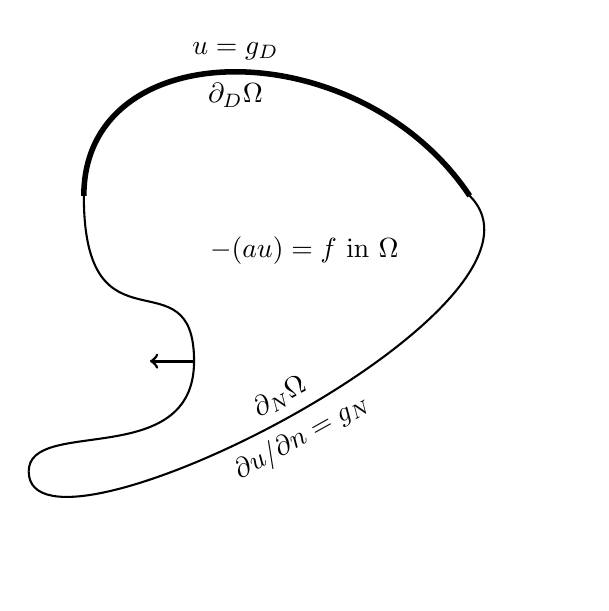
\begin{tikzpicture}[scale=0.7]
%\draw[gray,very thin] (-2,-6) grid (8,3);
\draw[line width=2pt] (0,0) .. controls (0,3) and (5,3) .. node[sloped,above] {$u=g_D$} node[sloped,below] {$\partial_D\Omega$} (7,0);
\draw[line width=0.75pt] (7,0) .. controls (9,-2) and (-1,-7) .. node[sloped,above] {$\partial_N\Omega$} node[sloped,below] {$\partial u/\partial n = g_N$} (-1,-5);
\draw[line width=0.75pt] (-1,-5) .. controls (-1,-4) and (2,-5) .. (2,-3);
\draw[line width=0.75pt] (2,-3) .. controls (2,-1) and (0,-3) .. (0,0);
\draw[->,line width=1.0pt] (2,-3) -- (1.2,-3) node[below] {$\bn$}; % normal vector
\draw (4,-1) node {$- \Div (a \grad u) = f$ in $\Omega$};
\end{tikzpicture}


\caption{Problem \eqref{eq:un:poissonstrong} on a domain.}
\label{fig:un:generalpoissondomain}
\end{marginfigure}

Let $\Omega \subset \RR^2$ be a bounded (open) region.  Suppose its boundary $\partial\Omega$ is well-behaved (polygonal or Lipschitz-continuous \citep[section 1.2]{Ciarlet2002}).  Suppose $\partial\Omega$ is decomposed into (measurable) disjoint subsets $\partial_D \Omega$ and $\partial_N \Omega$ whose union is the entire boundary $\partial \Omega$.

The Poisson problem in Chapter \ref{chap:st} is based on the equation $- \grad^2 u = f$.  We allow a more general nonlinear form here.  Let $a(x,y,u)$ and $f(x,y,u)$ be continuous functions, and assume there is $\eps>0$ so that
    $$a(x,y,u) \ge \eps > 0.$$
That is, we require \emph{uniform ellipticity} \citep{Evans2010}.  The strong form also includes boundary conditions, here nonhomogeneous Dirichlet and Neumann boundary conditions.  Thus the  nonlinear Poisson (diffusion) \emph{strong form} we solve is to find $u(x,y)$ so that
\begin{align}
- \Div \left(a(x,y,u) \grad u\right) &= f(x,y,u) \quad \text{ on } \Omega, \label{eq:un:poissonstrong} \\
u &= g_D \quad \text{ on } \partial_D \Omega, \notag \\
\frac{\partial u}{\partial n} &= g_N \quad \text{ on } \partial_N \Omega. \notag
\end{align}
By definition, $\partial u/\partial n = \bn \cdot \grad u$ where $\bn$ is the outward unit normal on $\partial \Omega$.

The data of problem \eqref{eq:un:poissonstrong}, besides the region $\Omega$ and its boundary, includes a \emph{diffusion coefficient} $a$, a \emph{source term} $f$, \emph{Dirichlet data} $g_D$, and \emph{Neumann data} $g_N$.  For the purpose of numerical solutions we will simply assume that the boundary data is continuous.  Poisson problem \eqref{poissonsquare} in Chapter \ref{chap:st} is the homogeneous Dirichlet case where $\Omega$ is the square, $a\equiv 1$, $f=f(x,y)$ is independent of the solution $u$, $\partial_D \Omega = \partial \Omega$, $\partial_N \Omega = \emptyset$, and $g_D=0$.

Problem \eqref{eq:un:poissonstrong} is not the most general (nonlinear) Poisson problem.  Specifically, one could allow more general \emph{Robin} boundary conditions $\alpha u + \beta \frac{\partial u}{\partial n} = \gamma$ where, generally, $\alpha,\beta,\gamma$ could vary along the boundary \citep{Elmanetal2005}.  One could also allow $a$ and/or $f$ to depend on the gradient of $u$, as does $a=|\grad u|^{p-2}$ in the $p$-Laplacian equation of Chapter \ref{chap:of}.

As \eqref{eq:un:poissonstrong} is stated there may be no solution where ``$\Div(a\grad u)$'' makes sense as a continuous function, even for polygonal regions and continuous data.  That is, there may be no $u\in C^2(\Omega) \cap C(\overline \Omega)$ so that $-\Div(a\grad u) = f$.  A solution exists, however, in the linear case at least, if we convert \eqref{eq:un:poissonstrong} to a \emph{weak form}.  A weak formulation arose in Chapter \ref{chap:of} as the gradient of an objective function, but the weak form here is generally not of that type.  We will derive it from the strong form in the traditional way, by multiplying by a test function and integrating.


\section{Weak form with general boundary values}

Recall $L^2(\Omega)$ is the space of square-integrable real functions on $\Omega$.  Define the following Sobolev space \citep{Evans2010}:
    $$H^1(\Omega) = \left\{u \,:\, u \in L^2(\Omega) \,\&\, \grad u \in L^2(\Omega)\right\}.$$
Definition \eqref{eq:of:sobolevdefn} of $W^{1,p}(\Omega)$ includes this space so that $H^1(\Omega) = W^{1,2}(\Omega)$.  This Chapter uses the notation with ``$H$'' standing for Hilbert.

We use two subsets of $H^1(\Omega)$: \emph{trial functions} come from $H_{g}^1(\Omega)$, which denotes the functions with value $g_D$ along $\partial_D \Omega$, and \emph{test functions} come from $H_{0}^1(\Omega)$, with value $0$ along $\partial_D \Omega$.  Note that $H_{0}^1(\Omega)$ is a linear subspace of $H^1(\Omega)$ while generally $H_{g}^1(\Omega)$ is not.

Now choose any $v\in H_{0}^1(\Omega)$, multiply the first equation in \eqref{eq:un:poissonstrong} by $v$, and integrate by parts:
\begin{equation*}
\int_\Omega a(u) \grad u \cdot \grad v - \int_{\partial\Omega} \frac{\partial u}{\partial n} v = \int_\Omega f(u) v.
\end{equation*}
(In writing such integrals we generally show dependence on the solution $u$ but suppress it for $x,y$ so that $a(x,y,u)=a(u)$, and similarly for $f$.)  Next we use the boundary information, namely that $v=0$ on $\partial_D\Omega$ and $\frac{\partial u}{\partial n}=g_N$ on $\partial_N\Omega$:
\begin{equation}
\int_\Omega a(u) \grad u \cdot \grad v = \int_\Omega f(u) v + \int_{\partial_N\Omega} g_N v\quad \text{ for any } v\in H_{0}^1(\Omega). \label{eq:un:poissonweak}
\end{equation}
Equation \eqref{eq:un:poissonweak} is the \emph{weak formulation} of \eqref{eq:un:poissonstrong}, and any $u \in H_{g}^1(\Omega)$ satisfying it is a \emph{weak solution}.  Observe that the Dirichlet boundary conditions $g_D$ are incorporated into defining $H_{g}^1(\Omega)$ while the Neumann boundary data $g_N$ appears in the weak form \eqref{eq:un:poissonweak}.

Summarizing the ``rules'' for passing between the strong \eqref{eq:un:poissonstrong} and weak \eqref{eq:un:poissonweak} formulations might clarify the situation:\begin{itemize}
\item A well-behaved function $u \in C^2(\Omega) \cap C(\overline \Omega)$ which satisfies the strong form also solves the weak form.  (The derivation above shows this.)
\item If $u \in H_{g}^1(\Omega)$ solves the weak form then we accept it, by definition, as a solution.   If it is also well-behaved (i.e.~$u \in C^2(\Omega) \cap C(\overline \Omega)$) then we may reverse the derivation to show it solves the strong form.  (Not shown, but see \citet{Evans2010}.)
\end{itemize}

Consider the linear case where functions $a$ and $f$ are independent of $u$.  If $\partial_D \Omega$ has positive measure then a solution to weak formulation \eqref{eq:un:poissonweak} exists and is unique (\emph{well-posedness}; \citep{Ciarlet2002,Evans2010}).  There exist conditions on the domain (e.g.~convex polygon) and the boundary data under which one can furthermore show that $u$ solving \eqref{eq:un:poissonweak} is in $C^2(\Omega) \cap C(\overline \Omega)$ (\emph{regularity}; \citep{Evans2010}).  Such theoretical matters are mostly beyond our scope.

In nonlinear cases each particular problem must be analyzed for well-posedness.  In terms of practical computation, particular nonlinear cases covered by our method, and solvable using our code, include 2D versions of
\begin{itemize}
\item the \emph{Bratu} equation\sidenote{Exercises \ref{chap:nl}.\ref{exer:nl:bratu} and \ref{chap:un}.\ref{exer:un:bratu} solve the 1D and 2D versions, respectively.} if $a\equiv 1$ and $f=\lambda e^u$, and
\item ``uniformized'' versions of the \emph{porous medium} equation \citep{Ockendonetal2003}, in which, for example, $a=u^{m-1}+\eps$ for some $m\ge 1$ and $\eps>0$.
\end{itemize}


\section{A $P^1$ FEM}

A FEM for the Poisson problem comes from requiring the weak formulation \eqref{eq:un:poissonweak} to be true for $u$ in a finite-dimensional subspace of $H_{g}^1(\Omega)$, and for test functions $v$ ranging over a basis of a finite-dimensional subspace of $H_{0}^1(\Omega)$.\sidenote{An FEM is \emph{conforming} if these subspace claims are accurate.  Otherwise one is guilty of \emph{variational crimes} \citep{Ciarlet2002} with \emph{nonconforming elements} \citep{Braess2007}.}  In the \emph{Galerkin} method here, these subspaces, built upon a triangulation of $\Omega$, will be nearly the same.

To make our test function space $H_{0}^1(\Omega)$ a true subspace of $H^1(\Omega)$ we require that $\Omega$ be polygonal, with $\partial\Omega$ a closed polygon (Figure \ref{fig:un:polygon}).  Furthermore we require that segments which form the polygon $\partial\Omega$ be either entirely in $\partial_D\Omega$ or entirely in $\partial_N\Omega$.

We will assume $\partial_D\Omega$ is a closed set.  Furthermore we assume it contains at least one segment of positive length.  As suggested above, this leads to well-posedness of the continuum problem, at least in the linear case.

\begin{marginfigure}
\input{tmp/blob.tikz}
\caption{A polygonal domain $\Omega$.  The Dirichlet portion of the boundary $\partial_D\Omega$ is shown in bold.}
\label{fig:un:polygon}
\end{marginfigure}

By definition, a \emph{triangulation} is a finite set of non-overlapping, non-empty open triangles $\triangle_k\subset \RR^2$ which tile $\Omega$:
\begin{equation}
\Th = \left\{\triangle_k \,\Big|\, \cup_k \overline{\triangle}_k = \overline{\Omega} \, \text{ and} \,\, \Omega_k \cap \Omega_l = \emptyset \, \text{ if } k\ne l\right\}. \label{eq:un:triangulation}
\end{equation}
We index the $K$ triangles (elements) in $\Th$ by $k=0,\dots,K-1$.  The $N$ vertices (nodes) in $\Th$ are indexed by $j=0,1,\dots,N-1$, with locations
\begin{equation*}
\bx_j = (x_j,y_j).
\end{equation*}

An example triangulation $\Th$ is shown in Figure \ref{fig:un:number-mesh}.  The subscript ``$h$'' in ``$\Th$,'' traditional notation, denotes the typical or maximum size $h$ (e.g.~diameter) of the triangles.  It serves as a reminder of our desired limit $h\to 0$.  In contrast to many references--e.g.~\citet{Elmanetal2005}, which we follow in many ways---all numbering here is zero-based, suitable for a C implementation.

We will use $P^1$ finite elements \citep{Elmanetal2005} so that our test and trial functions are continuous and linear on each $\triangle_k$.  On each triangle $\triangle_k$, such functions have three degrees of freedom.  We make think of these as the coefficients in the linear formula $a + b x + c y$, but in fact there are better local bases than $\{1,x,y\}$; see below.

For each node $j$ there is a basis (``hat'') function  $\psi_j(x,y)$ which is linear on each triangle, continuous on all of $\overline{\Omega}$, and equal to one at only one node $j$,
\begin{equation*}
\psi_j(\bx_i) = \delta_{ij}.
\end{equation*}
See Figure \ref{fig:un:hatfunction}.  (Compare Figure \ref{fig:of:q1hat}.)  Functions $\psi_j$ are in $H^1(\Omega)$ \citep{Braess2007}, with piecewise-constant partial derivatives $\partial\psi_j/\partial x$ and $\partial\psi_j/\partial y$.  The set $\{\psi_j\}_{j=0,\dots,N-1}$ is linearly-independent.

\begin{marginfigure}
\input{tmp/blob.1.elenum.tikz}

\medskip

\input{tmp/blob.1.nodenum.tikz}
\caption{A triangulation of the polygon in Figure \ref{fig:un:polygon}, with element (top) and node (bottom) numbering.  There are $K=15$ elements, $N=13$ nodes, and $n_D=4$ nodes in $\partial_D\Omega$.}
\label{fig:un:number-mesh}
\end{marginfigure}

Hat functions allow us to interpolate and extend the Dirichlet data $g_D$ from its node values in $\partial_D \Omega$ to the whole of $\overline\Omega$, a useful step in our FEM implementation.  We number the $n_D$ nodes which are in the Dirichlet boundary by $\bx_{j_l} \in \partial_D\Omega$ for $l=0,\dots,n_D-1$.  (Figure \ref{fig:un:number-mesh} shows $n_D=4$ and $j_l=l$.)  Now let $\hat g_D \in C(\overline\Omega)$ be the piecewise-linear interpolant of $g_D$ which has value zero at all nodes $\bx_j$ which are not in the Dirichlet boundary $\partial_D \Omega$:
\begin{equation}
\hat g_D(x,y) = \sum_{l=0}^{n_D-1} g_D(\bx_{j_l}) \psi_{j_l}(x,y). \label{eq:un:hatgdefine}
\end{equation}

We can specify the needed finite-dimensional subspaces in terms of $\hat g_D$ and the span of certain basis functions $\psi_j$.  The \emph{test functions} are zero along $\partial_D \Omega$,
\begin{align*}
S_{0}^h &= \Span\left<\psi_j \,:\, \bx_j \notin \partial_D \Omega\right> = \Span\left<\psi_j \,:\, j \neq j_l\right>.
\end{align*}
The \emph{trial functions} have value $g_D$ along $\partial_D \Omega$,
\begin{equation}
S_{g}^h = \left\{\hat g_D + w \,:\, w \in S_{0}^h\right\}.
\end{equation}
Note that $S_{0}^h$ is a linear subspace of $H_{0}^1(\Omega)$ while $S_{g}^h$ is merely an affine subspace of $H^1(\Omega)$.  Also
\begin{equation}
\dim(S_{0}^h)=\dim(S_{g}^h)=N-n_D.
\end{equation}

\begin{marginfigure}
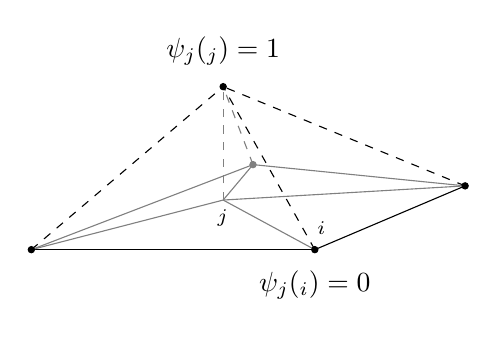
\begin{tikzpicture}[scale=0.9, z={(.707,.3)}]
    % (2,2,1) is top
    \draw[style=dashed] (0,0,0) -- (2,2,1); % to top from left
    \draw[style=dashed] (4,0,0) -- (2,2,1); %   ...  from front
    \draw[style=dashed] (4,0,3) -- (2,2,1); %   ...  from right
    \draw[color=gray, style=dashed] (0.3,0,4) -- (2,2,1); % from back
    \draw[color=gray, style=dashed] (2,0.4,1) -- (2,2,1); % from middle
    % draw base
    \draw (0,0,0) -- (4,0,0);
    \draw (4,0,0) -- (4,0,3);
    \draw[color=gray] (0,0,0) -- (0.3,0,4);
    \draw[color=gray] (0.3,0,4) -- (4,0,3);
    \draw[color=gray] (0,0,0) -- (2,0.4,1);
    \draw[color=gray] (2,0.4,1) -- (4,0,3);
    \draw[color=gray] (4,0,0) -- (2,0.4,1);
    \draw[color=gray] (2,0.4,1) -- (0.3,0,4);
    % draw \psi_j at nodes
    \filldraw (2,2,1) circle (1.25pt);
    \draw (2,2.5,1) node {$\psi_j(\bx_j)=1$};
    \draw (2,0.15,1) node {$\bx_j$};
    \filldraw (0,0,0) circle (1.25pt);
    \filldraw (4,0,0) circle (1.25pt);
    \draw (4,-0.5,0) node {$\psi_j(\bx_i)=0$};
    \draw (4.1,0.3,0) node {$\bx_i$};
    \filldraw (4,0,3) circle (1.25pt);
    \filldraw[color=gray] (0.3,0,4) circle (1.25pt);
\end{tikzpicture}


\caption{Hat functions $\psi_j$.}
\label{fig:un:hatfunction}
\end{marginfigure}

The FEM itself can now be stated.  It requires \eqref{eq:un:poissonweak} to be true for $u^h\in S_{g}^h$ for all $v^h\in S_{0}^h$.  However, it suffices to consider $v^h$ from a basis of $S_{0}^h$, so we require
\begin{equation}
\int_\Omega a(u^h) \grad u^h \cdot \grad \psi_i = \int_\Omega f(u^h) \psi_i + \int_{\partial_N\Omega} g_N \psi_i \label{eq:un:weakformhat}
\end{equation}
for all $i$ such that $\bx_i \notin \partial_D \Omega$.  On the other hand we may expand $u^h$ using $N-n_D$ unknown coefficients $u_j\in\RR$:
\begin{equation}
u^h(x,y) = \hat g_D(x,y) + \sum_{\bx_j \notin \partial_D \Omega} u_j\, \psi_j(x,y). \label{eq:un:uhexpand}
\end{equation}

The coefficients $u_j$ in \eqref{eq:un:uhexpand} are the unknowns.  Given the triangulation $\mathcal{T}_h$ of $\Omega$ and the data of the problem, namely the functions $a$, $f$, $g_D$, and $g_N$, the complete specification of the FEM solution $u^h$ is given by equations \eqref{eq:un:hatgdefine}, \eqref{eq:un:weakformhat}, and \eqref{eq:un:uhexpand}.

In the linear case it is common to now write system \eqref{eq:un:weakformhat} and \eqref{eq:un:uhexpand} as a linear system $A \bu = \bb$.  The usual next step in an FEM is to assemble the \emph{stiffness matrix} $A$ \citep{Elmanetal2005}.  However, we will not do so until we have an initial, and verified, numerical solution.  Following the pattern established since Chapter \ref{chap:nl}, we first implement equation \eqref{eq:un:weakformhat} as a residual-evaluation function $\bF(\bu)$, from the representation of $u^h$ as a vector $\bu$.  In evaluating $\bF$ we use \eqref{eq:un:uhexpand} to get point values of $u^h$ and its gradient $\grad u^h$ on the interior of triangles.  These point values allow quadrature, similar to that in Chapter \ref{chap:of}, to approximate the integrals in \eqref{eq:un:weakformhat}.  Implementing a residual in the linear case is mathematically equivalent to assembling $A$ and $\bb$, but the residual-evaluation code here is simpler because it does not require direct contact with a \pMat object at all.

In the next section we describe and the code the element-wise ``assembly,'' that is, evaluation of, the residual function $\bF$, as a \pSNES call-back.  However, before that can be written we need to be more specific about what \eqref{eq:un:weakformhat} says on each element.  Also we will read-in the triangular mesh and put it into \PETSc data structures.  These tools can be tested for correctness with a finite-differenced Jacobian (Chapter \ref{chap:nl}).  Once this is all shown to work correctly, via comparison to an exact solution, then we will re-consider matrix assembly, namely for the Jacobian derivative of $\bF$.


\section{Assembly of the residual equations}

Expression \eqref{eq:un:uhexpand} shows that $N-n_D$ real values $\{u_j\}$, for $j$ such that $\bx_j \notin \partial_D \Omega$, are needed to determine the FEM solution $u^h$.  However, it will be easier to write code if we \emph{increase} the size of the resulting nonlinear system, up to dimension $N$, by including the values of $u^h$ at nodes in the Dirichlet boundary as unknowns.  Thus we define
\begin{equation}
\bu = \{u_j\}_{j=0}^{N-1} \in \RR^N  \label{eq:un:unknowns}
\end{equation}
as the description of the FEM solution.

To enforce the boundary conditions, the components of the residual corresponding to Dirichlet boundary must be zero:
\begin{equation}
F_i(\bu) = u_i - g_D(\bx_i) \qquad \text{ if } \bx_i \in \partial_D\Omega.  \label{eq:un:dirichletresiduals}
\end{equation}

Because triangulation $\mathcal{T}_h$ satisfying \eqref{eq:un:triangulation} almost\sidenote{The set $\Omega \setminus \cup_k \triangle_k$ has measure zero.} covers $\Omega$ with non-overlapping triangles, we can write the weak form \eqref{eq:un:weakformhat} as a sum over elements.  To be specific, for each $\triangle_k \in \mathcal{T}_h$, $k=0,\dots,K-1$, let
\begin{equation}
F_i^k(\bu) = \int_{\triangle_k} a(u^h) \grad u^h \cdot \grad \psi_i - f(u^h) \psi_i.  \label{eq:un:elementweakform}
\end{equation}
Suppose $n_N$ is the number of edges which are in the Neumann boundary.  We call these edges (Neumann) \emph{segments} for distinctive language.  For each segment $s_\nu$, $\nu=0,\dots,n_N-1$, let
\begin{equation}
\varphi_i^\nu = \int_{s_\nu} g_N \psi_i,  \label{eq:un:segmentweakform}
\end{equation}
and note that $\varphi_i^\nu$ does not depend on the solution $u^h$.  Then residual equation \eqref{eq:un:weakformhat} is
\begin{equation}
F_i(\bu) = \sum_{k=0}^{K-1} F_i^k(\bu) - \sum_{\nu=0}^{n_N-1} \varphi_i^\nu = 0  \qquad \text{ if } \bx_i \notin \partial_D\Omega. \label{eq:un:elementwisesum}
\end{equation}
Together, equations \eqref{eq:un:dirichletresiduals} and \eqref{eq:un:elementwisesum} form the (generally) nonlinear system, of dimension $N$, which we supply to the \pSNES solver:
\begin{equation}
\bF(\bu)=0. \label{eq:un:fullsystem}
\end{equation}

Observe that $n_D$ is the number of \emph{nodes} in the Dirichlet boundary, whereas $n_N$ is the number of \emph{segments} (edges) in the Neumann boundary.  The former correspond to degrees of freedom, while the latter are domains of integration.  Managing the mesh correctly requires making this distinction.

Because the support of the hat function $\psi_i$ only overlaps with a few triangles $\triangle_k$, only a few values $F_i^k(\bu)$ and $\varphi_i^\nu$ are nonzero.  Also, only a few nodal values $\bu=\{u_j\}$ enter into $F_i^k(\bu)$, namely those values $u_j$ such that the support of $\psi_j$ overlaps with $\triangle_k$.  These facts make \eqref{eq:un:fullsystem} a \emph{sparse} nonlinear system.

We will compute the element integrals \eqref{eq:un:elementweakform} by referring $\triangle_k$ to a reference triangle $\triangle_\ast$ with vertices $(0,0),\,(1,0),\,(0,1)$, as shown in Figure \ref{fig:isoparametric}.  In Chapter \ref{chap:of} we did the same thing for quadrilaterals, so now we can be brief.

If $\triangle_k$ has vertices $(x_0,y_0),\,(x_1,y_1),\,(x_2,y_2)$ then the linear map from $\triangle_\ast$ to $\triangle_k$ is
\begin{align}
x(\xi,\eta) &= x_0 + (x_1-x_0) \xi + (x_2-x_0) \eta, \label{eq:un:trianglemap} \\
y(\xi,\eta) &= y_0 + (y_1-y_0) \xi + (y_2-y_0) \eta. \notag
\end{align}
The Jacobian determinant of map \eqref{eq:un:trianglemap}, needed for change-of-variables to integrate over the reference element, is constant on each element.  Its magnitude is the ratio of the area of $\triangle_k$ to the area of the reference element $\triangle_\ast$, equal to $2|\triangle_k|$ because $|\triangle_\ast|=1/2$.  See Exercise \ref{chap:un}.\ref{exer:un:gradientdetails}.

\begin{marginfigure}
\begin{tikzpicture}[scale=1.1,
    decoration={
      markings,
      mark=at position 1 with {\arrow[scale=1.8,gray]{latex}};
    }]
% left x,y axes
    \draw[->, gray, very thin] (1.5,0) -- (4.0,0);
    \draw[->, gray, very thin] (2,-0.5) -- (2,2.4);
    \draw (4.1,-0.1) node {$x$};
    \draw (1.9,2.4) node {$y$};
    \filldraw (1.7,1) circle (1.25pt);    % (x_0,y_0)
    \filldraw (3.5,-0.3) circle (1.25pt); % (x_1,y_1)
    \filldraw (3.0,2.0) circle (1.25pt);  % (x_2,y_2)
    \draw (1.4,1.3) node {$(x_0,y_0)$};
    \draw (3.5,-0.6) node {$(x_1,y_1)$};
    \draw (3.0,2.3) node {$(x_2,y_2)$};
    \draw[line width=1pt] (1.7,1) -- (3.5,-0.3) -- (3.0,2.0) -- cycle;
    \draw (2.7,1.0) node {$\triangle_k$};
% right xi,eta axes
    \draw[->, gray, very thin] (4.6,0) -- (6.6,0);
    \draw[->, gray, very thin] (5,-0.4) -- (5,2.0);
    \draw (6.7,-0.1) node {$\xi$};
    \draw (4.9,2.05) node {$\eta$};
    \filldraw (5,0) circle (1.25pt);  % (0,0)
    \filldraw (6,0) circle (1.25pt);  % (1,0)
    \filldraw (5,1) circle (1.25pt);  % (0,1)
    \draw (5.2,-0.3) node {$0$};
    \draw (6.2,0.2) node {$1$};
    \draw (5.2,1.1) node {$2$};
    \draw[line width=1pt] (5,0) -- (6,0) -- (5,1) -- cycle;
    \draw (5.3,0.3) node {$\triangle_\ast$};
% arrows connecting nodes
    \draw[gray, postaction={decorate}] (5,0) -- (1.7,1.03);
    \draw[gray, postaction={decorate}] (6,0) -- (3.5,-0.3);
    \draw[gray, postaction={decorate}] (5,1) -- (3.0,2.0);
\end{tikzpicture}


\caption{Mapping of a triangle $\triangle_k$ from the reference triangle $\triangle_\ast$.}
\label{fig:isoparametric}
\end{marginfigure}

On $\triangle_\ast$ any linear function is a linear combination of three local (nodal) basis functions:
\begin{equation}
\chi_0(\xi,\eta) = 1-\xi-\eta, \qquad \chi_1(\xi,\eta) = \xi, \qquad \chi_2(\xi,\eta) = \eta. \label{eq:un:chiformulas}
\end{equation}
If $\bx_i\in\overline{\triangle_k}$ then hat function $\psi_i$ satisfies
\begin{equation}
\psi_i(x(\xi,\eta),y(\xi,\eta)) = \chi_\ell(\xi,\eta) \label{eq:un:psichimap}
\end{equation}
for all $(\xi,\eta)\in\triangle_\ast$, where vertex $\ell \in \{0,1,2\}$ of $\triangle_\ast$ maps to $\bx_i$.

Recalling both the change-of-variables formula for integrals and the chain rule, we can write
\begin{equation}
F_i^k(\bu) = 2 |\triangle_k| \int_{\triangle_\ast} H_\ell^k(\bu,\xi,\eta)\,d\xi\,d\eta \label{eq:un:elementintegralreference}
\end{equation}
where the integrand is
\begin{equation}
H_\ell^k(\bu,\xi,\eta) = \left[a(u^h) \grad u^h \cdot \grad \psi_i - f(u^h) \psi_i\right]_{\triangle_\ast}.  \label{eq:un:elementintegrand}
\end{equation}
Here vertex $\ell$ of $\triangle_\ast$ corresponds to the node $\bx_i$.  Note that ``$\grad$'' in \eqref{eq:un:elementintegrand} refers to derivatives in variables $x,y$.  Exercises \ref{chap:un}.\ref{exer:un:gradientdetails} and \ref{chap:un}.\ref{exer:un:elementintegranddetails} addresses the details implicit in \eqref{eq:un:elementintegralreference} and \eqref{eq:un:elementintegrand}.

As in Chapter \ref{chap:of}, the integrals \eqref{eq:un:elementintegralreference} will be approximated using quadrature.  Generally, if there are $Q$ quadrature points $(\xi_q,\eta_q) \in \triangle_\ast$ with weights $w_q$ then
\begin{equation}
F_i^k(\bu) \approx 2 |\triangle_k| \sum_{q=0}^{Q-1} w_q H_\ell^k(\bu,\xi_q,\eta_q). \label{eq:un:elementquadraturereference}
\end{equation}
We use symmetric quadrature rules constructed for the reference triangle $\triangle_\ast$.\sidenote{Unsymmetric quadrature rules based on tensor products of one-dimensional integrals \citep{KarniadakisSherwin2013} are an alternative.}  Table \ref{tab:un:quadrature} shows degree $1,2,3$ Gaussian rules \citep{Dunavant1985} with $Q=1,3,4$ points, respectively (Exercise \ref{chap:un}.\ref{exer:un:checkquadrature}).  Note that the sum of the weights is $1/2$ because $|\triangle_\ast|=1/2$.

\begin{table}[h]
\vspace{0.1in}

\begin{tabular}{lccc}
degree & $Q$ & weights $w_q$ & nodes $(\xi_q,\eta_q)$ \\ \hline
$1$ & $1$ & $1/2$ & $(1/3,1/3)$ \\ \hline
$2$ & $3$ & \begin{tabular}{c}
            $1/6$ \\
            $1/6$ \\
            $1/6$
            \end{tabular} & \begin{tabular}{c}
            $(1/6,1/6)$ \\
            $(2/3,1/6)$ \\
            $(1/6,2/3)$
            \end{tabular} \\ \hline
$3$ & $4$ & \begin{tabular}{c}
            $-27/96$ \\
            $25/96$ \\
            $25/96$ \\
            $25/96$
            \end{tabular} & \begin{tabular}{c}
            $(1/3,1/3)$ \\
            $(1/5,1/5)$ \\
            $(3/5,1/5)$ \\
            $(1/5,3/5)$
            \end{tabular}
\end{tabular}

\vspace{0.1in}
\caption{Symmetric quadrature rules on the reference triangle $\triangle_\ast$.  See \eqref{eq:un:elementquadraturereference}.} \label{tab:un:quadrature}
\end{table}

For the Neumann boundary contributions we use the midpoint rule.  Observe that hat function $\psi_i$ has value $1/2$ at the midpoint of any edge which is incident to $\bx_i$.  Thus
\begin{equation}
\varphi_i^\nu \approx g_N(x_m,y_m) \psi_i(x_m,y_m) |s_\nu| = \frac{1}{2} |s_\nu|\, g_N(x_m,y_m), \label{eq:un:segmentquadrature}
\end{equation}
if $\bx_i \in \overline{s_\nu}$, and it is zero otherwise.  Here $(x_m,y_m)$ is the midpoint, and $|s_\nu|$ is the length, of segment $s_\nu$.


\section{Example problems}

Let us set up some cases on a trapezoidal domain, with known exact solutions, for testing the FEM.  The first two cases are designed to test the implementation of the PDE and of Dirichlet boundary conditions.  One of these problems is linear and the other is nonlinear.  An additional case tests the non-homogeneous Neumann boundary condition implementation.  These cases are about as simple as possible given that they test the important parts of our code (below).  That is, we the errors from the FEM will only converge a the theoretical rate $O(h^2)$ if our implementation is correct.

All three cases are based on manufactured solutions.  Let
\begin{equation}
  u_{\text{exact}}(x,y) = 1 - y^2 - \frac{1}{4} y^4. \label{eq:un:exactsolution}
\end{equation}
This function also computes the Dirichlet boundary values $g_D(x,y)$ in all cases.  Because the domain is not aligned with the coordinate axes, and because fourth-order polynomials generate non-zero interpolation errors in a $P^1$ FEM, the numerical error generated with this exact solution will decay no more rapidly than the generic rate.

\begin{figure}
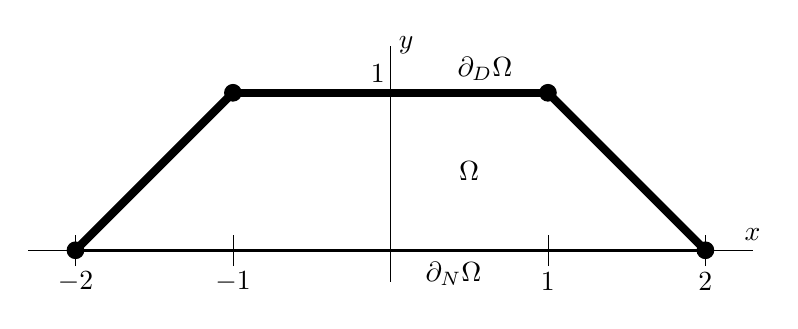
\begin{tikzpicture}[scale=2.000000]
% originally created, in part, by script tri2tikz.py command line:
%   tri2tikz.py --polyonly --nodesize 1.0 --scale 2.0 ../c/ch8/meshes/trap tmp/trap.tikz
% with by-hand edits
  \draw[thin] (0.0,-0.2) -- (0.0,1.3);
  \draw[thin] (-2.3,0.0) -- (2.3,0.0);
  \node at (2.3,0.1) {$x$};
  \node at (0.1,1.3) {$y$};
  \node at (0.5,0.5) {$\Omega$};
  \node at (-0.08,1.12) {$1$};
  \draw[very thin] (-2.0,-0.1) -- (-2.0,0.1);
  \node at (-2.0,-0.2) {$-2$};
  \draw[very thin] (-1.0,-0.1) -- (-1.0,0.1);
  \node at (-1.0,-0.2) {$-1$};
  \draw[very thin] (1.0,-0.1) -- (1.0,0.1);
  \node at (1.0,-0.2) {$1$};
  \draw[very thin] (2.0,-0.1) -- (2.0,0.1);
  \node at (2.0,-0.2) {$2$};
  \node at (0.4,-0.15) {$\partial_N \Omega$};
  \node at (0.6,1.15) {$\partial_D \Omega$};
  \draw[line width=3.0pt] (2.000000,0.000000) -- (1.000000,1.000000);
  \draw[line width=3.0pt] (1.000000,1.000000) -- (-1.000000,1.000000);
  \draw[line width=3.0pt] (-1.000000,1.000000) -- (-2.000000,0.000000);
  \draw[line width=1.25pt] (-2.000000,0.000000) -- (2.000000,0.000000);
  \filldraw (2.0,0.0) circle (1.5pt);
  \filldraw (1.0,1.0) circle (1.5pt);
  \filldraw (-1.0,1.0) circle (1.5pt);
  \filldraw (-2.0,0.0) circle (1.5pt);
\end{tikzpicture}

\caption{Exact solution cases $0$ and $1$ solve Poisson equations on a trapezoidal region $\Omega$.  Boundary subsets $\partial_D\Omega$, $\partial_N \Omega$ are as indicated.  See \texttt{trap.poly} in Code \ref{code:trappoly}.}
\label{fig:un:trap}
\end{figure}

Other details are case-specific:
\begin{itemize}
\item[case $0$:] \emph{Linear}.  Use Figure \ref{fig:un:trap} boundary conditions.  Noting $\partial u_{\text{exact}}/\partial n = \partial u_{\text{exact}}/\partial y = 0$ on the Neumann boundary $\partial_N \Omega$, where $y=0$, let $g_N=0$.  Let $a=1$ and determine $f$ by differentiating the exact solution: $f(x,y) = -\grad^2 u_{\text{exact}} = 2 + 3 y^2$.
\item[case $1$:] \emph{Nonlinear}.  Again use Figure \ref{fig:un:trap} boundary conditions and $g_N=0$.  However, let $a(u) = 1+u^2$ and compute the corresponding $f(u)$ by differentiation.
\item[case $2$:] \emph{Non-homogeneous Neumann}.  Use Figure \ref{fig:un:trapneu} boundary conditions.  Let $a$, $f$ be as in case $0$.  Determine the (non-zero) value $g_N$ by differentiating $u_{\text{exact}}$ along the Neumann boundary, a line segment with outward unit normal vector $\bn = \left<1/\sqrt{2},1/\sqrt{2}\right>$.
\end{itemize}
See \texttt{c/\CODELOC cases.h} (not shown) for all remaining details.

\begin{figure}
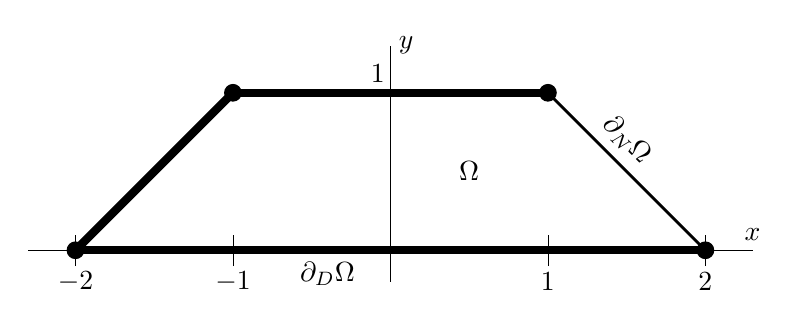
\begin{tikzpicture}[scale=2.000000]
% originally created, in part, by script tri2tikz.py command line:
%   tri2tikz.py --polyonly --nodesize 1.0 --scale 2.0 ../c/ch8/meshes/trap tmp/trap.tikz
% with by-hand edits
  \draw[thin] (0.0,-0.2) -- (0.0,1.3);
  \draw[thin] (-2.3,0.0) -- (2.3,0.0);
  \node at (2.3,0.1) {$x$};
  \node at (0.1,1.3) {$y$};
  \node at (0.5,0.5) {$\Omega$};
  \node at (-0.08,1.12) {$1$};
  \draw[very thin] (-2.0,-0.1) -- (-2.0,0.1);
  \node at (-2.0,-0.2) {$-2$};
  \draw[very thin] (-1.0,-0.1) -- (-1.0,0.1);
  \node at (-1.0,-0.2) {$-1$};
  \draw[very thin] (1.0,-0.1) -- (1.0,0.1);
  \node at (1.0,-0.2) {$1$};
  \draw[very thin] (2.0,-0.1) -- (2.0,0.1);
  \node at (2.0,-0.2) {$2$};
  \node at (-0.4,-0.15) {$\partial_D \Omega$};
  \node[rotate=-45] at (1.5,0.7) {$\partial_N \Omega$};
  \draw[line width=1.0pt] (2.000000,0.000000) -- (1.000000,1.000000);
  \draw[line width=3.0pt] (1.000000,1.000000) -- (-1.000000,1.000000);
  \draw[line width=3.0pt] (-1.000000,1.000000) -- (-2.000000,0.000000);
  \draw[line width=3.0pt] (-2.000000,0.000000) -- (2.000000,0.000000);
  \filldraw (2.0,0.0) circle (1.5pt);
  \filldraw (1.0,1.0) circle (1.5pt);
  \filldraw (-1.0,1.0) circle (1.5pt);
  \filldraw (-2.0,0.0) circle (1.5pt);
\end{tikzpicture}

\caption{Case $2$ uses the same region as in cases $0$ and $1$, but with different boundary conditions.  See \texttt{c/\CODELOC meshes/trapneu.poly} (not shown).}
\label{fig:un:trapneu}
\end{figure}


\section{Triangulations from \Triangle}

\PETSc does not include tools for triangulating regions of the plane, that is, for the initial generation of an unstructured mesh.  We use the widely-available \Triangle\sidenote{See \href{http://www.cs.cmu.edu/~quake/triangle.html}{www.cs.cmu.edu/$\sim$quake/ triangle.html} for documentation.} software \citep{Shewchuk1996} for this task.  \Triangle is limited to 2D, but the ASCII files it generates have straightforward details.

\Triangle inputs an ASCII file, with extension \texttt{.poly}, describing a polygonal region along with integer flags to indicate special vertices or segments on the boundary.  For example, the input file \texttt{trap.poly} (Code \ref{code:trappoly}) generates the polygon shown in Figure \ref{fig:un:trap}.

\inputwhole{../c/\CODELOC/meshes/trap.poly}{\CODELOC meshes/trap.poly}{A description of the boundary polygon in Figure \ref{fig:un:trap}, suitable for reading by \Triangle.}{code:trappoly}

The triangulation shown in Figure \ref{fig:un:trapone} came from applying \Triangle to \texttt{trap.poly}.  We ask for a polygon output file (option \texttt{-p}), relatively-uniform triangles (\texttt{-q} for ``quality-checked,'' with no interior angles less than $20^\circ$ \citep{Shewchuk1996}), and triangles with a maximum area (\texttt{-a}) of $0.5$:
\begin{cline}
$ cd c/ch7/meshes
$ triangle -pqa0.5 trap
\end{cline}
%$
This command generates three ASCII files, \texttt{trap.1.node}, \texttt{trap.1.ele}, and \texttt{trap.1.poly}; see Codes \ref{code:traponenode}--\ref{code:traponepoly}.  They define the new node locations, elements as triples of node indices, and segments in the polynomial boundary as pairs of node indices, respectively.  This triangulation has $N=8$ nodes, $K=6$ elements, $P=8$ boundary segments, $n_D=5$ Dirichlet nodes, and $n_N=4$ segments in the Neumann boundary.

\begin{figure}
\input{tmp/trap.1.tikz}
\caption{The triangulation described by \texttt{trap.1.\{node,ele,poly\}}.}
\label{fig:un:trapone}
\end{figure}

By giving value ``$2$'' to the Dirichlet nodes in the original \texttt{trap.poly} input, and because \Triangle itself uses ``$0$'' for non-boundary and ``$1$'' for otherwise un-flagged boundary nodes, we have this boundary flag scheme:
\begin{itemize}
\item[0] interior node,
\item[1] Neumann boundary node or segment, and
\item[2] Dirichlet node or segment.
\end{itemize}
Observe that, though \texttt{trap.poly} describes the boundary using only 4 segments, additional boundary nodes and segments have been added in generating the triangulation.

\inputwhole{misc/trap.1.node}{\CODELOC meshes/trap.1.node}{\Triangle-generated ASCII file for node locations and nodal boundary flags.}{code:traponenode}

\inputwhole{misc/trap.1.ele}{\CODELOC meshes/trap.1.ele}{\Triangle-generated ASCII file with element index triples.}{code:traponeele}

\inputwhole{misc/trap.1.poly}{\CODELOC meshes/trap.1.poly}{\Triangle-generated ASCII file for the refined polygon, including segment boundary flags.}{code:traponepoly}

We will test the FEM on a sequence of refined grids generated by \Triangle.  For an example, the command
\begin{cline}
$ triangle -rpqa0.1 trap.1
\end{cline}
%$
generates ASCII files \texttt{trap.2.\{node,ele,poly\}} with $N=33$ nodes, $K=33$ elements, and $P=19$ boundary segments (Figure \ref{fig:un:traptwo}).  Refinement (\texttt{-r}) here means that \emph{nodes} in the \texttt{trap.1} files are retained, but there is no such inclusion relationship for the edges or triangles.  We also see that the symmetry of the \texttt{trap.1} mesh was merely fortuitous.  Symmetries in the input polygon are not preserved by the \Triangle algorithms.

\begin{figure}
\input{tmp/trap.2.tikz}
\caption{A refined triangulation.}
\label{fig:un:traptwo}
\end{figure}

\Triangle includes a minimal visualization tool.  The command
\begin{cline}
$ showme trap
\end{cline}
%$
displays the boundary polygon from \texttt{trap.poly} and levels of the triangulation (\texttt{trap.\{1,2\}.\{node,ele,poly\}}).


\section{From ASCII files to \PETSc \pVecs and \pISs}

Our plan is to traverse the lists of elements $\triangle_k \in \mathcal{T}_h$, and Neumann boundary segments $s_\nu$, so as to compute the residuals $F_i(\bu)$ from equations \eqref{eq:un:elementquadraturereference} and \eqref{eq:un:segmentquadrature}, respectively.  The traversal is fast if the mesh data are stored in \PETSc objects, so we first convert the above \Triangle-generated ASCII files into \pVecs and \pISs using a Python script \texttt{tri2petsc.py}.

An abstract description clarifies the data types.  There are two kinds of ``data'' to describe a mesh, \emph{geometrical} and \emph{topological}.  Here the geometry is simply the location, a pair of real numbers, for all the nodes.  For simplicity we store these $x$ and $y$ coordinates as separate length $N$ (sequential) \pVecs.  For the topology we need descriptions of which elements (triangles) are incident to which nodes (vertices).  This task only requires integer indices as we refer to a node simply by a global index into the coordinate \pVecs for $x$ and $y$.  Thus the topology of the elements is given by providing a triple of integers, in the range $0,\dots,N-1$, for each element.  Similarly, a segment of the polygonal boundary is simply a pair of nodal indices referring to the endpoints.

The \PETSc \pIS ``index set'' type is convenient for storing these indices.  The reader may regard an \pIS simply as an ``integer-valued \pVec'' in the current use.\sidenote{In this Chapter we do not exploit the ``main purpose'' of an \pIS in distributed (multi-process) indexing.}  The \pIS storing the element index triples holds $3K$ integers and the \pIS for boundary segments holds $2P$ integers.

Some care is needed in recording the Dirichlet and Neumann parts of the boundary.  First, one cannot tell if an edge in the triangulation is a boundary segment just from whether the endpoints are in the boundary.\sidenote{For example, the edge from node 5 to node 7 in Figure \ref{fig:un:number-mesh} is not a boundary segment.}  Second, the endpoints of a boundary segment could be nodes in the (closed) Dirchlet boundary, while the segment itself is in the (relatively-open) Neumann boundary.  Therefore, despite the apparent redundancy, we will separately store flags for the \emph{nodes}, indicating whether they are interior ($0$) or Neumann boundary ($1$) or Dirichlet boundary ($2$), and for the \emph{segments} on the boundary, either $1$ for Neumann or $2$ for Dirichlet.  This scheme is the one used by \Triangle.  Two more \pISs are used to store these flags.

Thus the Python script \texttt{tri2petsc.py} (not shown) reads three files in \Triangle-generated ASCII format, as described above, with extensions \texttt{.node,.ele,.poly}.  Then it writes two files in \PETSc binary format with extensions \texttt{.vec,.is}.  The first output file holds two \pVecs with the node coordinates.  The second output file holds four \pISs (element triples, nodal boundary flags, boundary segment pairs, and boundary segment flags).

Let's try it out.  Because \texttt{tri2petsc.py} uses Python modules from the \PETSc source directory, we first generate some symbolic links:
\begin{cline}
$ cd c/ch7/
$ ln -s ~/petsc/bin/petsc_conf.py
$ ln -s ~/petsc/bin/PetscBinaryIO.py
$ ./tri2petsc.py meshes/trap.1 trap.1
\end{cline}
This generates two files \texttt{trap.1.vec} and \texttt{trap.1.is}.  Our C code will then load these binary data with \PETSc functions  \texttt{VecLoad()} and \texttt{ISLoad()}, respectively.

It is convenient for the C code to have a data structure for all mesh information, so we define a new \texttt{UM} (``unstructured mesh'') data type, a C \texttt{struct}.  See Code \ref{code:umstruct}.  Of course, this \texttt{UM} data type is superceded by advanced, \PETSc-supported tools in Chapter \ref{chap:dp}.

\cinput{um.h}{\CODELOC}{An unstructured-mesh data type.}{//STARTUM}{//ENDUM}{code:umstruct}

Admittedly-tedious C functions \texttt{UMInitialize()}, \texttt{UMDestroy()}, \texttt{UMView()}, \texttt{UMReadVecs()}, and \texttt{UMReadISs()} in \texttt{c/\CODELOC um.c} (not shown) have the task of reading \texttt{.vec,.is} binary files and allocating/filling/destroying a \texttt{UM} instance.

\section{Initial implementation}

With an unstructured mesh in hand we can return to implementing the FEM.  We build the minimal \pSNES-using C code which works, called \texttt{c/\CODELOC unfem.c}.  In its initial implementation it has a ``context'' \texttt{struct}, which includes a \texttt{UM} instance, a residual-computation function \texttt{FormFunction()}, and a \texttt{main()} function.  The latter reads options and then creates\sidenote{And destroys at the end.} a \pSNES and \pVecs for holding the approximate solution, the exact solution, and the residual.  For the FEM itself we need enough information to transfer integrals to the reference triangle, and we need quadrature data structures, so we set these up.  There is then nothing else to do, other than to call \texttt{SNESSolve()}.  Figure \ref{fig:un:unfemstack} shows the structure of \texttt{unfem.c}, including the approximate Jacobian (implementation shown later).

Before showing this code, and because the reader might have become too comfortable with \pDMDA-using structured-grid examples in recent Chapters, recalling the first example in Chapter \ref{chap:nl} might be appropriate.  In terms of \PETSc objects and calls to the \PETSc API, \texttt{unfem.c} has a similar structure to \texttt{ecjac.c} in Chapter \ref{chap:nl}.

\begin{figure}
\begin{tikzpicture}[scale=0.8,
                    >={Latex[length=2mm]},
  component/.style={
     rectangle,draw,fill=white,align=center,line width=1pt},
  userfcn/.style={
     rounded corners,draw,fill=white,draw,align=center,line width=1pt,font={\itshape,\normalsize}}]

\draw[line width=1pt] (3,7) node[userfcn,minimum width=105mm] (usercode) {user code \\ \vspace{15mm}};

\draw[line width=1pt] (0,7.2) node[userfcn] (rescode) {residual \emph{\texttt{FormFunction()}}};
\draw[line width=1pt] (5.2,6.2) node[userfcn] (jaccode) {approximate Jacobian \emph{\texttt{FormPicard()}}};

\draw[line width=1pt] (-1,4) node[component] (snes) {\complabel{\pSNES}{nonlinear solver}};
\draw[line width=1pt] (-1,2) node[component] (ksp)  {\complabel{\pKSP}{linear solver}};
\draw[line width=1pt] (-1,0) node[component] (pc)   {\complabel{\pPC}{preconditioner}};

\draw[line width=1pt] (2,2) node[component] (matj)   {\usedlabel{\pMat}{Jacobian}};
\draw[line width=1pt] (3.5,0) node[component] (vecs)   {\pVecs \\ \footnotesize  \emph{solution, other fields}};
\draw[line width=1pt] (7.5,0) node[component] (iss)   {\pISs \\ \footnotesize  \emph{node indices, bdry flags}};

\path
   ([xshift=-10em]usercode.south) edge[->] node {} (snes)
   ([xshift=0em]usercode.south) edge[->] node {} ([xshift=2em]vecs.north)

   (rescode.south) edge[->,bend left] node {} (vecs.north)
   ([xshift=-2em]rescode.south) edge[->] node {} (iss.north)

   (jaccode.south) edge[->] node {} (matj)
   ([xshift=2em]jaccode.south) edge[->] node {} ([xshift=4em]vecs.north)
   ([xshift=4em]jaccode.south) edge[->] node {} ([xshift=2em]iss.north)

   (snes) edge node {} (ksp)
   (ksp) edge node {} (pc);
\end{tikzpicture}
\caption{The \PETSc object structure of \texttt{unfem.c}.}
\label{fig:un:unfemstack}
\end{figure}


FIXME show extracts of context, FEM stuff, most of \texttt{FormFunction()}, and most of \texttt{main()} in \texttt{c/\CODELOC unfem.c}

\cinputpart{unfem.c}{\CODELOC}{FIXME}{I}{//STARTCTX}{//ENDCTX}{code:unfemctx}

\cinputpart{unfem.c}{\CODELOC}{FIXME}{II}{//STARTFEM}{//ENDFEM}{code:unfemfem}

\cinputpart{unfem.c}{\CODELOC}{FIXME}{III}{//STARTBDRYRESIDUALS}{//ENDBDRYRESIDUALS}{code:unfembdryresiduals}

\cinputpart{unfem.c}{\CODELOC}{FIXME}{IV}{//STARTELEMENTRESIDUALS}{//ENDELEMENTRESIDUALS}{code:unfemelementresiduals}

\cinputpart{unfem.c}{\CODELOC}{FIXME}{V}{//STARTMAIN}{//ENDMAIN}{code:unfemmain}


\section{Initial testing}

FIXME demo convergence with \texttt{-snes\_fd}


\section{Assembling an approximate Jacobian}

FIXME EXPLAIN PICARD $\bF(\bu)=0$ to $A(\bu) \bu - \bb(\bu)=0$ to $A(\bu^k) \bu^{k+1} - \bb(\bu^k)=0$ to $A(\bu^k) (\bu^{k+1}-\bu^k) - \bb(\bu^k)= - A(\bu^k) \bu^k$ to $A(\bu^k) \bs = -\bF(\bu^k)$  The linear system at a step, $A(\bu^k) \bs = -\bF(\bu^k)$, has $A=A(\bu^k)\in\RR^{N\times N}$ and $\bb=-\bF(\bu^k)\in\RR^N$, where $N$ is the number of nodes.  \pMat and \pVec objects store the problem, and, unlike in the \texttt{-snes\_fd} and \texttt{-snes\_mf} cases used above, wherein the \pMat object stayed invisibly inside the \pSNES solver, we now assemble the \pMat.

FIXME by considering \eqref{eq:un:dirichletresiduals}, \eqref{eq:un:elementweakform}, and \eqref{eq:un:elementwisesum}, the entries of this Picard/Jacobian matrix are
\begin{equation}
A_{ij}(\bu) =  \begin{cases}
               1, & i \in \partial_D\Omega \text{ or } j \in \partial_D\Omega, \\
               \sum_{k=0}^{K-1} A_{ij}^k(\bu), & \text{otherwise},
               \end{cases} \label{eq:un:picardentry}
\end{equation}
where
\begin{equation}
A_{ij}^k(\bu) = \int_{\triangle_k} a(u^h) \grad\psi_j \cdot \grad\psi_i \label{eq:un:picardentryelement}
\end{equation}
Again this is computed by quadrature, similar to \eqref{eq:un:elementintegralreference} and \eqref{eq:un:elementquadraturereference}.  This matrix is evidently symmetric, $a_{ij}=a_{ji}$, and sparse.  Furthermore it is positive-definite if $a(u,x,y)>0$, and thus the conjugate gradient Krylov method applies to the equations for the Newton step; see Chapter \ref{chap:ls}.

\cinputpart{unfem.c}{\CODELOC}{FIXME}{VI}{//STARTPICARD}{//ENDPICARD}{code:unfempicard}


\section{Preallocate a \pMat (serial)}

FIXME essential for speed

\cinputpart{unfem.c}{\CODELOC}{FIXME}{VII}{//STARTPREALLOC}{//ENDPREALLOC}{code:unfemprealloc}

compare for \texttt{--with-debugging=0} build:
\begin{cline}
$ timer ./unfem -un_mesh meshes/trap.7 -un_noprealloc
case 0 result for N=46421 nodes:  |u-u_exact|_inf = 6.55365e-05
real 56.30
$ timer ./unfem -un_mesh meshes/trap.7
case 0 result for N=46421 nodes:  |u-u_exact|_inf = 6.55365e-05
real 0.97
\end{cline}

\section{Performance relative to \pDMDA structured grid}

FIXME introduce \texttt{genstructured.py} and case 3; compares well in serial to Chapter 3 example

compare for \texttt{--with-debugging=0} build (note $1025^2=1050625$):
\begin{cline}
$ cd c/ch3/
$ make poisson
$ timer ./poisson -da_refine 7 -ksp_type cg -pc_type icc
on 1025 x 1025 grid:  error |u-uexact|_inf = 5.29691e-08
real 18.67
$ cd ../ch7
$ ./genstructured.py meshes/square.10 1025
$ ./tri2petsc.py meshes/square.10 meshes/square.10
$ make unfem
$ timer ./unfem -un_mesh meshes/square.10 -un_quaddeg 1 -un_case 3
case 3 result for N=1050625 nodes:  |u-u_exact|_inf = 9.89813e-08
real 24.47
\end{cline}

\section{Next steps}

FIXME: parallel approach could use \Triangle \texttt{.neigh} file as adjacency graph for elements, run \texttt{MatPartitioning} stuff (see manual), apply partitioning to get \pIS (or \texttt{AO}), and have nodes and edges follow along

FIXME: paraphrase Barry: The ``trick'' is that first partition the element across processes, then partition the vertices (nodal values) subordinate to the partitioning of the elements and then you renumber the elements and vertices so that the elements on the first process are numbered first, followed by the elements on the second process etc and similarly the vertices on the first process are numbered before the vertices on the second processes etc.  Each process loops over its elements computing the element stiffness/load and calling \texttt{MatSetValues/VecSetValues()} using the ``new'' numbering of the vertices.  The ``old'' numbering that was on the disk is not used in communicating with PETSc.

FIXME: see approach to mesh topology in chapter 10 of \citep{Loggetal2012}


\section{Exercises}

\renewcommand{\labelenumi}{\arabic{chapter}.\arabic{enumi}\quad}
\renewcommand{\labelenumii}{(\alph{enumii})}
\begin{enumerate}
\item  \label{exer:un:gradientdetails}  For the map \eqref{eq:un:trianglemap} from $\triangle_\ast$ to $\triangle_k$, let
    $$J_k = \frac{\partial (x,y)}{\partial (\xi,\eta)} = \begin{pmatrix}
    x_1 - x_0 & x_2 - x_0 \\
    y_1 - y_0 & y_2 - y_0 \end{pmatrix}
    = \begin{pmatrix}
    \Delta x_1 & \Delta x_2 \\
    \Delta y_1 & \Delta y_2
    \end{pmatrix}$$
be the Jacobian.  Use the chain rule and \eqref{eq:un:psichimap} to show that
\begin{equation}
\grad_{x,y} \psi_i = \frac{1}{\det J_k} \left<\Delta y_2 \frac{\partial \chi_\ell}{\partial \xi} - \Delta y_1 \frac{\partial \chi_\ell}{\partial \eta}, - \Delta x_2 \frac{\partial \chi_\ell}{\partial \xi} + \Delta x_1 \frac{\partial \chi_\ell}{\partial \eta}\right>. \label{eq:un:gradpsionref}
\end{equation}
Here indices $i$ and $\ell$ have the same relationship as in \eqref{eq:un:psichimap}.  Comparing formula \eqref{eq:of:gradpsionref} for the structured case, what is the underlying reason why \eqref{eq:un:gradpsionref} is a bit more complicated?  % underlying reason is that affine map here includes rotations, while in Chapter \ref{chap:of} it was just translation and axes scaling
\item  \label{exer:un:elementintegranddetails}  Formula \eqref{eq:un:elementintegrand} might require some interpretation before the implementation becomes clear.  Confirm that, with only mild abuses of notation, formulas \eqref{eq:un:trianglemap} and \eqref{eq:un:psichimap} lead to the valid expansions
\begin{align*}
a(u^h) &= a(u^h,\xi,\eta) = a(u^h,x(\xi,\eta),y(\xi,\eta)), \\
f(u^h) &= f(u^h,\xi,\eta) = f(u^h,x(\xi,\eta),y(\xi,\eta)), \\
\psi_i &= \chi_{\ell}(\xi,\eta), \\
u^h &= \sum_{j=0}^{N-1} \left\{\begin{matrix} g_D(\bx_j) \\ u_j \end{matrix}\right\} \chi_{\ell'}(\xi,\eta), \\
\grad u^h &= \grad_{x,y} u^h = \sum_{j=0}^{N-1} \left\{\begin{matrix} g_D(\bx_j) \\ u_j \end{matrix}\right\} \grad_{x,y} \psi_j.
\end{align*}
For the third formula, node $\bx_i$ corresponds to vertex $\ell$ on $\triangle_\ast$.  In the fourth and fifth formulas, node $\bx_j$ corresponds to vertex $\ell'$ on $\triangle_\ast$, and the two cases for the coefficient are when $\bx_j \in \partial_D \Omega$ and $\bx_j \notin \partial_D \Omega$, respectively.  Note that \eqref{eq:un:gradpsionref} allows us to expand $\grad_{x,y} \psi_j$ in the fifth formula.  Taken together, these expansions make \eqref{eq:un:elementintegrand} meaningful and implementable.
\item  \label{exer:un:checkquadrature}  The degree of accuracy $n=1,2,3$ of the quadrature rules in Table \ref{tab:un:quadrature} can be checked by comparing the exact integral
\begin{equation}
\iint_{\triangle_\ast} \xi^i \eta^j\,d\xi d\eta = \frac{i!\,j!}{(i+j+2)!}, \label{eq:un:checkquadrature}
\end{equation}
for all cases with $0\le i+j\le n$, against the quadrature result.  Also one should show an inexact quadrature result for some case with $i+j=n+1$.  Write a small program, in the language of your choice, which does these things.
\item \label{exer:un:basisfreeresidual} FIXME motivated by \citep{Loggetal2012}: replace $\bF(\bu)$ with $\bF(\bu;v)$ so that residual equation no longer requires basis of $S^h$ for its definition; advantages/disadvantages?
\item \label{exer:un:truejacobian} FIXME implement the true Jacobian in the $a=a(x,y)$ case, so that we only add a diagonal $\partial f/\partial u$ term; test on case 1 example and see if improved \pSNES convergence
\item \label{exer:un:bratu} FIXME using result from previous exercise, solve Bratu; compute critical $\lambda$; equals 6.81 according to \pSNES example \texttt{ex5.c}
\item \label{exer:un:gaussneumann}  In \texttt{unfem.c} we use the midpoint rule, the one-point Gauss rule, for quadrature \eqref{eq:un:segmentquadrature} computing the Neumann boundary segment contributions $\varphi_\nu^i$.  Modify \texttt{unfem.c} to optionally allow two-point Gaussian quadrature for this purpose.  Only in case 2 will this make any difference.  Show that accuracy improves for coarse grids, but that this benefit disappears under grid refinement.
% see c/ch7/solns/segmentgauss.c.snippet
\end{enumerate}

